% Author: Izaak Neutelings (July 2021)
% Description: summary of optical phenomena
\documentclass[border=3pt,tikz]{standalone}
\usetikzlibrary{arrows,arrows.meta}
\usetikzlibrary{calc}
\usetikzlibrary{decorations.markings}
\usetikzlibrary{angles,quotes} % for pic (angle labels)
\usetikzlibrary{intersections}
\usetikzlibrary{fadings}
%\usetikzlibrary{decorations.pathmorphing} % for snake lines
\tikzset{>=latex} % for LaTeX arrow head

\colorlet{myblue}{blue!80!black}
\colorlet{mydarkblue}{blue!35!black}
\colorlet{glasscol}{blue!10}
\tikzstyle{myarr}=[-{Latex[length=3,width=2]}]
\tikzstyle{glass}=[top color=glasscol!88!black,bottom color=glasscol,shading angle=0]
\tikzstyle{glassbulk}=[top color=glasscol!80!black,bottom color=glasscol!80!black,middle color=white,shading angle=0]
\tikzset{
  ray/.style={thick,myblue,decoration={markings,
                     mark=at position #1 with {\arrow{latex}}},
                     postaction={decorate}},
  ray/.default=0.5}
\tikzfading[name=fade out, 
    inner color=transparent!0,
    outer color=transparent!100]

\def\W{2.0} % width interface
\def\l{1.8} % length ray
\def\g{0.2} % depth glass gradient
\def\d{0.3} % glass depth
\def\glass{
  %\fill[glassbulk] (-\W/2,0) rectangle (\W/2,-\t); % glass bulk
  \fill[glasscol] (-\W/2,0) rectangle (\W/2,-\d); % glass bulk
  \fill[glass] (-\W/2,0) rectangle++ (\W,-\g*\d); % glass gradient
  \fill[glass,shading angle=180] (-\W/2,-\d) rectangle++ (\W,\g*\d); % glass gradient
}

\begin{document}


% TRANSMISSION
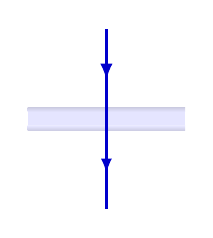
\begin{tikzpicture}
  \coordinate (O) at (0, 0);          % point of contact
  \coordinate (A) at (0,0.55*\l);     % point incident (top left)
  %\coordinate (M) at (0,-\d);        % point of exit (bottom)
  \coordinate (B) at (0,-\d-0.55*\l); % point refracted (bottom)
  \glass
  \draw[ray={0.65},line width=1.0] (A) -- (O); % incoming ray
  \draw[ray={0.65},line width=0.8] (O) -- (B); % refracted ray
  \fill[myblue] (O) circle(0.0175);
\end{tikzpicture}


% ABSORPTION
\begin{tikzpicture}
  \def\ang{30}
  \def\r{0.6*\d} % absorption radius
  \coordinate (O) at (  0, 0); % point of contact
  \coordinate (A) at (90+\ang:\l); % point incident (top left)
  \glass
  \draw[ray={0.55},line width=1.0] (A) -- (O); % incoming ray
  \fill[myblue] (O) circle(0.0175);
  \begin{scope}
    \clip (O) --++ (\r,0) arc(0:-180:\r) -- cycle;
    \fill[myblue,path fading=fade out,opacity=0.80]
      (O) circle(\r);
  \end{scope}
\end{tikzpicture}


% REFLECTION
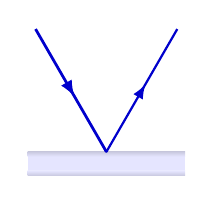
\begin{tikzpicture}
  \def\ang{30}
  \coordinate (O) at (  0, 0); % point of contact
  \coordinate (A) at (90+\ang:\l); % point incident (top left)
  \coordinate (B) at (90-\ang:\l); % point refracted (bottom)
  \glass
  \draw[ray={0.55},line width=1.0] (A) -- (O); % incoming ray
  \draw[ray={0.55},line width=0.8] (O) -- (B); % refracted ray
  \fill[myblue] (-0.0021,0.0055) circle(0.019);
\end{tikzpicture}


% REFRACTION
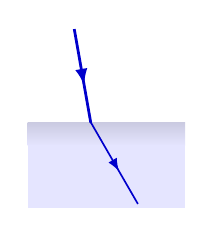
\begin{tikzpicture}
  \def\W{2.0} % width interface
  \def\l{1.2} % length ray
  \def\g{0.3} % depth glass gradient
  \def\d{0.8} % glass depth
  \def\f{0.4} % fraction
  \coordinate (O) at (0,0);    % point of contact
  \coordinate (A) at (100:\l); % point incident (top left)
  \coordinate (B) at (-60:\l); % point refracted (bottom)
  \fill[glass] (-\f*\W,0) rectangle++ (\W,-\g); % glass gradient
  \fill[glasscol] (-\f*\W,-0.99*\g) rectangle++ (\W,-\d); % glass bulk
  \draw[ray={0.60},line width=1.0] (A) -- (O); % incoming ray
  \draw[ray={0.60},line width=0.6] (O) -- (B); % refracted ray
  \fill[myblue] (O) circle(0.0175);
\end{tikzpicture}


% SCATTERING
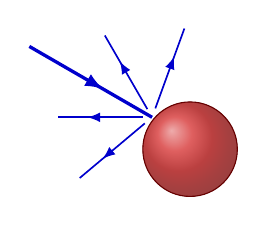
\begin{tikzpicture}
  \def\R{0.3*\W}
  \def\sl{0.6*\l} % length scattered ray
  \coordinate (I) at (140:1.05*\R); % point incident (top left)
  \coordinate (A) at ($(I)+(150:\l)$); % incoming ray origin
  \fill[ball color=red!80!black] (0,0) circle(\R);
  \draw[red!40!black,fill=red!80!black!50,fill opacity=0.5] (0,0) circle(\R);
  \draw[ray={0.6},line width=1.2] (A) -- (I); % incoming ray
  \foreach \angs in {70,120,180,220}{
    \draw[ray={0.65},line width=0.6] (I)++(\angs:0.2*\R) --++ (\angs:\sl); % scattered ray
  }
\end{tikzpicture}


% DIFFRACTION
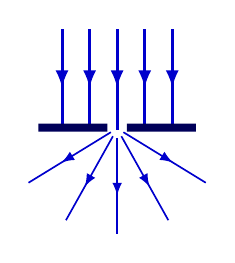
\begin{tikzpicture}
  \def\w{1.4}  % beam width
  \def\W{2.0}  % width interface
  \def\l{1.3}  % length ray
  \def\o{0.25} % opening width
  \def\t{0.1}  % wall thickness
  \def\N{5}    % number of incoming rays
  %\coordinate (O) at (0,0);  % point of contact
  %\coordinate (A) at (0,\l); % point incident (top left)
  \foreach \i [evaluate={\x=-\w/2+(\i-1)*\w/(\N-1);}] in {1,...,\N}{
    \draw[ray={0.58},line width=1.1] (\x,\l) --++ (0,-0.98*\l); % incoming rays
  }
  \foreach \ang in {-60,-30,0,30,60}{
    %\draw[ray={0.6},line width=0.6] (0,0) -- (\ang-90:\l); % outgoing ray
    \draw[ray={0.6},line width=0.6] (1.4*\ang-90:0.08) -- (\ang-90:\l); % outgoing ray
  }
  %\fill[myblue] (O) circle(0.0265);
  \fill[mydarkblue]
    (-\o/2,0) rectangle (-\W/2,\t)
    ( \o/2,0) rectangle ( \W/2,\t);
\end{tikzpicture}


\end{document}